
Linear Meld (LM) is a forward chaining logic programming language where a
program is defined by a \emph{database of facts} and by a set of
\emph{derivation rules}. LM supports structured manipulation of mutable state
through the use of linear logic~\cite{girard-87} by supporting two types of
logical facts, namely, \emph{persistent facts} (which cannot be retracted) and
\emph{linear facts} (which can be retracted).

LM programs are evaluated as follows. Initially, we populate the database with
the program's initial facts and then determine which derivation rules can be
applied by using the facts from the database. Once a rule is applied, we derive
new facts, which are then added to the database. If a rule uses linear facts,
they are consumed and thus deleted from the database. The program stops when we
reach \emph{quiescence}, that is, when we can no longer obtain new facts through
rule derivation.

LM views the database of facts as a graph data structure where each node contains
facts belonging to that node. The database of facts can also be seen as a
collection of node objects and each node contains several attributes represented
as facts that describe the node. Derivation rules are restricted so that they
are only allowed to manipulate facts belonging to the same node. This
restriction allows nodes of the graph to compute independently of other nodes
since they can only perform computation with their current attributes.
Communication between nodes arises when a rule derives a fact that belongs to
another node. These design decisions allow LM to be concurrent and to also avoid
the granularity problem that is usually present in declarative languages. Since
computation is performed locally at each node of the graph, it is possible to
group nodes into computation units that can processed independently by the same
processing thread, which allows the implementation to easily control the
granularity of the program.

\section{A Taste Of LM}

In order to understand how LM programs are written, we now present and discuss
three LM programs.

\subsection{First Example: Message Routing}\label{section:language:message}

Figure~\ref{code:language:message} shows the first LM program, a message routing
program that simulates message transmission through a network of nodes.
Lines~\ref{line:language:message_pred1}-\ref{line:language:message_pred2}
declare the predicates used in the program's rules. Note that the first argument
of every predicate must be typed as \code{node} because the first argument
indicates where the fact lives in the graph. Predicate \code{edge} is a
\emph{persistent predicate} while \code{message} and \code{processed} are
\emph{linear predicates}. Persistent predicates model facts that are never
retracted from the database, while linear predicates model linear facts which
are retracted when used in rules. To improve readability of LM rules, persistent
predicates are preceded with a \code{!} symbol. Predicate \code{edge} represents
the connections between nodes, predicate \code{message} contains the message
content and the route list, and predicate \code{processed} keeps count of the
number of messages routed at each node. Along with the type, a predicate
argument can also be named (e.g., see \code{Neighbor} and \code{Content}) for
documentation purposes.

\begin{figure}[h!]
\begin{Verbatim}[numbers=left,commandchars=\*\{\},fontsize=\codesize]
type edge(node, node Neighbor).*label{line:language:message_pred1}*hfill// Predicate declaration
type linear message(node, string Content, list node Routing).
type linear processed(node, int Total).*label{line:language:message_pred2}

message(A, Content, [B | L]),*label{line:language:message_first1}*hfill// Rule 1
!edge(A, B),
processed(A, N)
   -o processed(A, N + 1),
      message(B, Content, L).*label{line:language:message_first2}

message(A, Content, []),*label{line:language:message_second1}*hfill// Rule 2
processed(A, N)
   -o processed(A, N + 1).*label{line:language:message_second2}
\end{Verbatim}
\mycap{LM code for routing messages in a graph.}
\label{code:language:message}
\end{figure}

The message routing program in Fig.~\ref{code:language:message} implements two
rules. An LM rule has the form $L_1, \cdots, L_n \mathtt{-o} \; R_1, \cdots,
R_m$, where $L_1, \cdots, L_n$ is the \emph{left-hand side}~(LHS) of the rule
and $R_1, \cdots, R_m$ is \emph{right-hand side}~(RHS) of the rule. The meaning
of a rule is then as follows: if facts $L_1, \cdots, L_n$ are present in the
database then consume all the facts $L_i$ that are linear facts and derive the
facts $R_1, \cdots, R_m$ from the RHS. Note that in the rules, the LHS of each
rule uses only facts from the same node (represented by \code{A} in both rules
of Fig.~\ref{code:language:message}), but the rule's RHS may derive facts that
belong to other nodes (case of \code{B} in the first rule) if the variable is
instantiated in the LHS.

The first rule
(lines~\ref{line:language:message_first1}-\ref{line:language:message_first2})
grabs the head node \code{B} in the route list (third argument of \code{message}
using the syntax \code{[B | L]} to represent the head and tail of a list) and
ensures that a communication edge exists (through \code{edge(A,~B)}). If so, we
increase the number of processed messages by consuming \code{processed(A,~N)}
and then deriving \code{processed(A,~N~+~1)}, and by deriving a new message to
the head node \code{B}.  When the route list is empty, the message has reached
its destination and thus it is simply consumed (second rule in lines
\ref{line:language:message_second1}-\ref{line:language:message_second2}).

The initial facts of the program are presented in
Fig.~\ref{code:language:message_facts}. The \code{edge} facts describe the
structure of the graph, where the node in the first argument has a direct
connection with the node in the second argument. Node literals are represented
using the syntax \code{@N}, where \code{N} is an non-negative number. We also
declare the message that needs to be routed with the content \code{"hello
world"} and a route list with the nodes \code{@3} and \code{@4}.

\begin{figure}[h!]
\begin{Verbatim}[numbers=left,commandchars=\*\{\},fontsize=\codesize]
!edge(@1, @2). !edge(@2, @3).
!edge(@3, @4). !edge(@1, @3).
processed(@1, 0). processed(@2, 0).
processed(@3, 0). processed(@4, 0).
message(@1, "hello world", [@3, @4]).
\end{Verbatim}
\mycap{Initial facts for the message routing program. There is only one message ("hello
world") to route through nodes \code{@3} and \code{@4}.}
\label{code:language:message_facts}
\end{figure}

In Fig.~\ref{fig:message_trace} we present an execution trace of the message
routing program. The database is represented as a graph structure where the
edges represent the \code{edge} initial facts. To simplify the figure, we
dropped the first argument of each fact since the first argument corresponds to
the node where the fact is placed. In Fig.~\ref{fig:message_trace}(a) the
database is initialized with the program's initial facts. Note that the initial
\code{message} fact is instantiated at node \code{@1}. After applying rule 1, we
get the database represented in Fig.~\ref{fig:message_trace}(b), where the
message has been derived at node \code{@3}. After applying rule 1 again, the
message is then routed to node \code{@4} (Fig.~\ref{fig:message_trace}(c))
where it will be consumed (Fig.~\ref{fig:message_trace}(d)).

\newcommand{\visitsize}{0.38}

\begin{figure}[h]
        \centering
        \begin{subfigure}[b]{\visitsize\textwidth}
                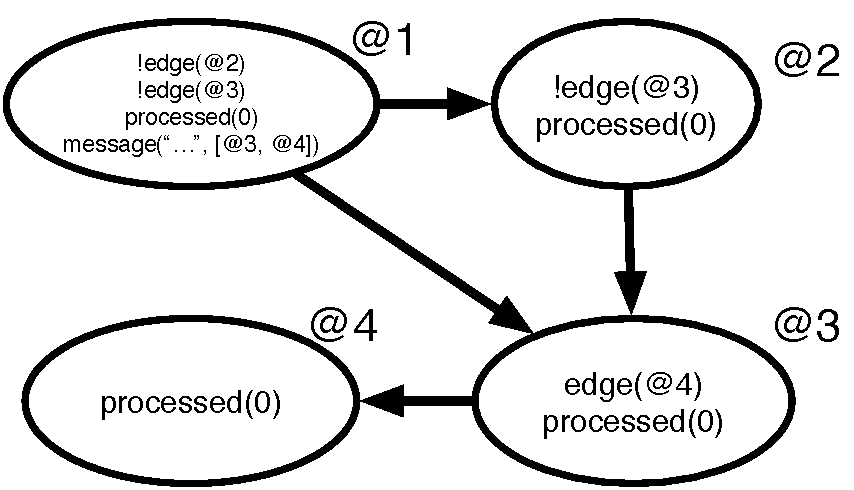
\includegraphics[width=\textwidth]{figures/message/message_trace1}
                \mycap{Initial database.}
                \label{fig:message_trace1}
        \end{subfigure}%
        ~
        \begin{subfigure}[b]{\visitsize\textwidth}
                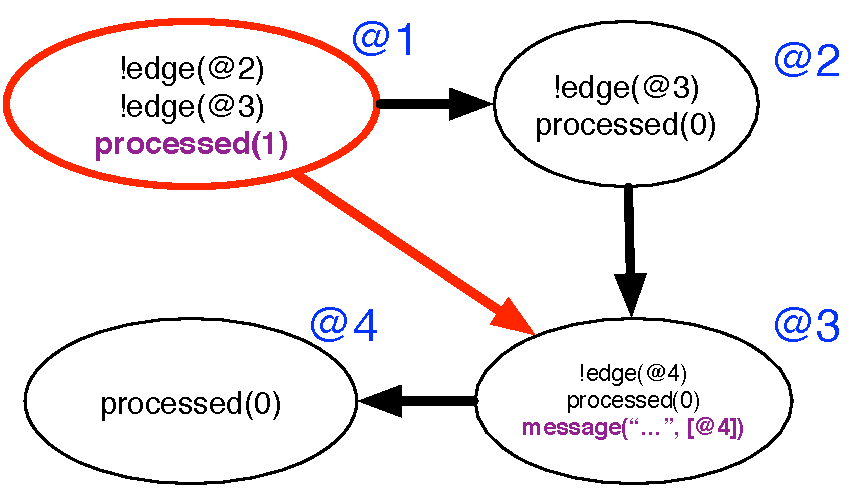
\includegraphics[width=\textwidth]{figures/message/message_trace2}
                \mycap{After applying rule 1 at node \code{@1}.}
                \label{fig:message_trace2}
        \end{subfigure}\\
        \begin{subfigure}[b]{\visitsize\textwidth}
                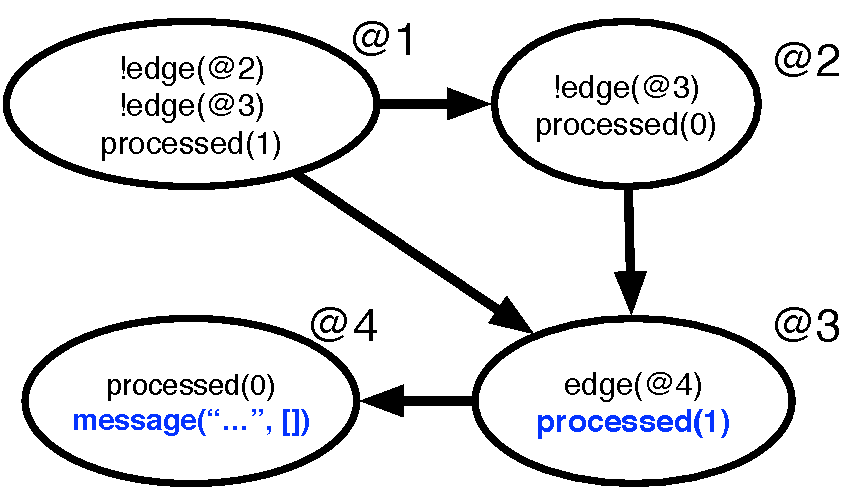
\includegraphics[width=\textwidth]{figures/message/message_trace3}
                \mycap{After applying rule 1 at node \code{@3}.}
                \label{fig:message_trace3}
        \end{subfigure}%
        ~
        \begin{subfigure}[b]{\visitsize\textwidth}
                  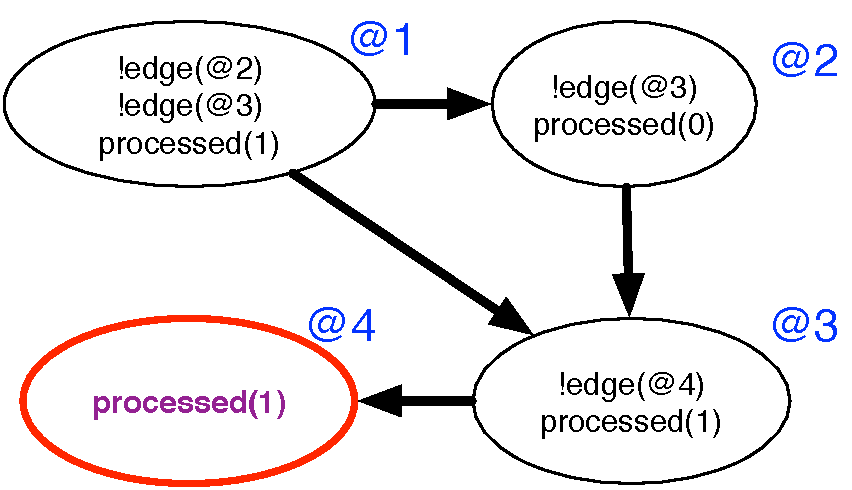
\includegraphics[width=\textwidth]{figures/message/message_trace4}
                  \mycap{After applying rule 2 at node \code{@4}.}
                  \label{fig:message_trace4}
          \end{subfigure}
        \mycap{An execution trace for the message routing program. The message "hello
        world" travels from node \code{@1} to node \code{@4}.}\label{fig:message_trace}
\end{figure}

The attentive reader will wonder how much concurrency is available in this
particular routing implementation. For a single message, there is no concurrency
because the message follows a pre-determined path and it travels from node to
node. However, concurrency arises when the program needs to route multiple
messages. The amount of concurrency is then dependent on the messages routing
lists being non-overlapping. If messages travel in different paths, then there
is more concurrency because more nodes are routing messages at the same time.


\subsection{Second Example: Key/Value Dictionary}\label{sec:language:key_value}

\begin{figure}[ht]
\begin{Verbatim}[numbers=right,fontsize=\codesize,commandchars=\*\{\}]
type left(node, node).*label{line:language:dict_header1}
type right(node, node).
type linear value(node, int Key, string Value).
type linear replace(node, int Key, string Value).*label{line:language:dict_header2}

replace(A, K, New),*label{line:language:dict_first1}
value(A, K, Old)
   -o value(A, K, New). // we found our key*label{line:language:dict_first2}

replace(A, RKey, RValue),*label{line:language:dict_second1}
value(A, Key, Value),
!left(A, B),
RKey < Key
   -o value(A, Key, Value),
      replace(B, RKey, RValue). // go left*label{line:language:dict_second2}

replace(A, RKey, RValue),*label{line:language:dict_third1}
value(A, Key, Value),
!right(A, B),
RKey > Key
   -o value(A, Key, Value),
      replace(B, RKey, RValue). // go right*label{line:language:dict_third2}

// initial configuration*label{line:language:dict_axioms1}
!left(@0, @1).     !right(@0, @2).
!left(@1, @3).     !right(@1, @4). 
!left(@2, @5).     !right(@2, @6).

value(@0, 3, "a").   value(@1, 1, "b").
value(@2, 5, "c").   value(@3, 0, "d").
value(@4, 2, "e").   value(@5, 4, "f").
value(@6, 6, "g").

// update key 6 to value "x"
replace(@0, 6, "x").*label{line:language:dict_axioms2}
\end{Verbatim}
\caption{LM program for replacing a key's value in a BST dictionary.}
\label{code:btree_replace}
\end{figure}

Our second example, shown in Fig.~\ref{code:btree_replace}, implements the key
update operation for a binary tree search~(BST) represented as a key/value
dictionary. Each LM node represents a binary tree node. We first declare all the
predicates in
lines~\ref{line:language:dict_header1}-\ref{line:language:dict_header2}.
Linear
predicate \texttt{value/3} assigns a key/value pair to a node that can be
updated later.  The \texttt{replace/3} linear predicate represents an update
operation where the key in the second argument will be updated to the value in
the third argument.

The algorithm uses three rules for the three possible cases of updating a key's
value: the first rule
(lines~\ref{line:language:dict_first1}-\ref{line:language:dict_first2}) performs
the update by removing \texttt{replace(A, K, New)} and \texttt{value(A, K, Old)}
and deriving \texttt{value(A, K, New)}; the second rule
(lines~\ref{line:language:dict_second1}-\ref{line:language:dict_second2})
recursively picks the left branch for the update operation by deleting
\texttt{replace(A, RKey, RValue)} and re-deriving it at node \texttt{B}; and the
third rule
(lines~\ref{line:language:dict_third1}-\ref{line:language:dict_third2}) picks
the right branch.
The initial facts of this program are presented in
lines~\ref{line:language:dict_axioms1}-\ref{line:language:dict_axioms2} and they
describe the initial binary tree configuration, including keys and values.  The
axiom \texttt{update(@0, 6, "x")} instantiated at the root node \texttt{@3}
manifests the intent to change the value of key 6 to 7.

Fig.~\ref{fig:btree_trace} represents the trace of the algorithm. The program
database is partitioned by the seven nodes using the first argument of each
fact. In Fig.~\ref{fig:btree_trace}~(a), we present the database filled with the
program's initial facts. Next, we follow the right branch using rule 3 since $6 > 3$
(Fig.~\ref{fig:btree_trace}~(b)).  We use the same rule again in
Fig.~\ref{fig:btree_trace}~(c) where we finally reach the key 6. Here, we apply
rule 1 and \texttt{value(@6, 6, "g")} is updated to \texttt{value(@6, 6, "x")}.

\begin{figure}[h]
        \centering
        \begin{subfigure}[b]{0.5\textwidth}
                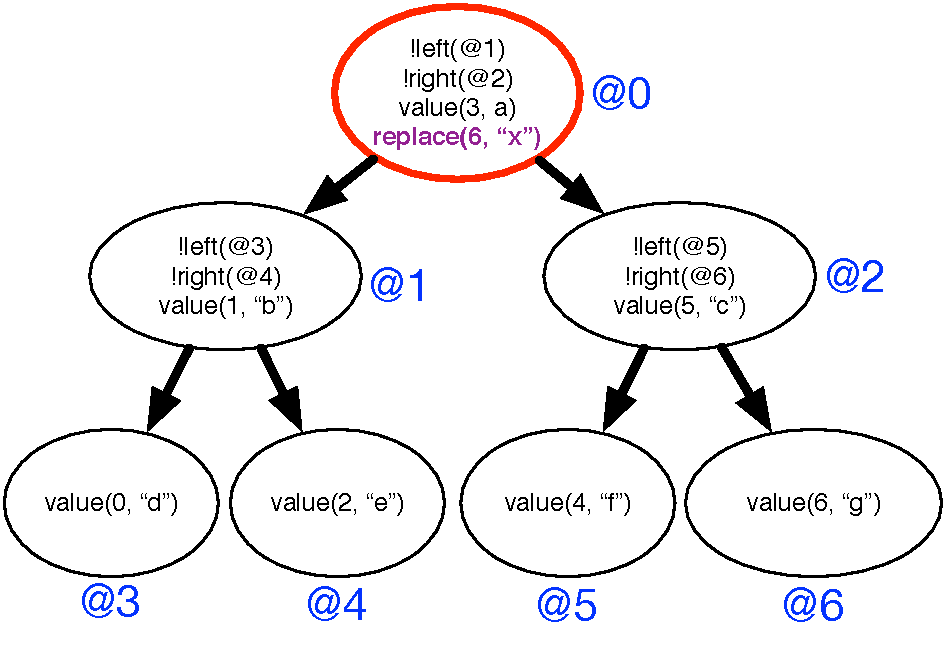
\includegraphics[width=\textwidth]{figures/btree/btree_trace1}
                \caption{Initial database. Replace axiom instantiated at the
                   \texttt{@3} root node.}
                \label{fig:btree_trace1}
        \end{subfigure}%
        ~
        \begin{subfigure}[b]{0.5\textwidth}
                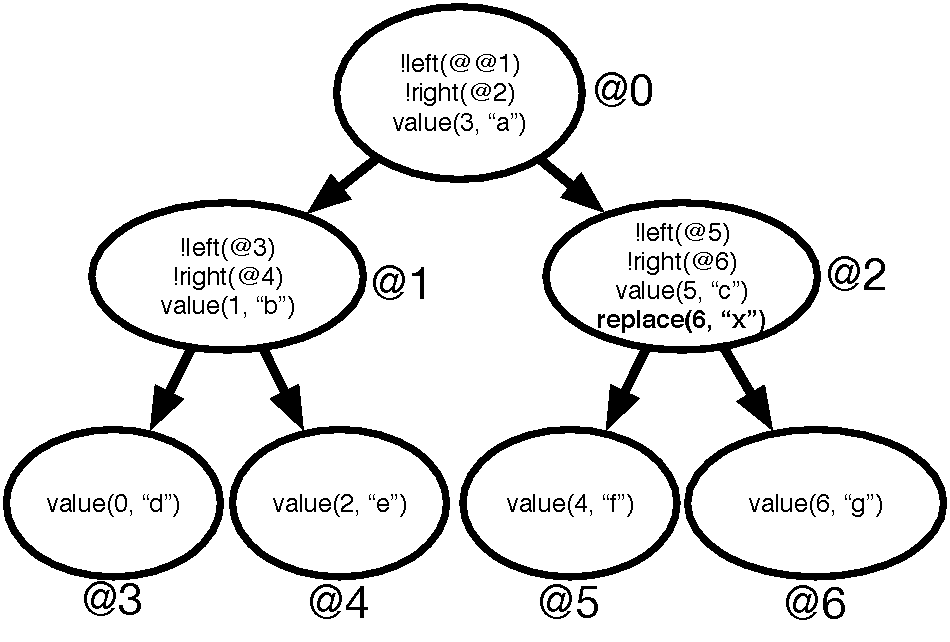
\includegraphics[width=\textwidth]{figures/btree/btree_trace2}
                \caption{After applying rule 3 at node \texttt{@3}. Replace fact
                   sent to node \texttt{@5}.}
                \label{fig:btree_trace2}
        \end{subfigure}\\
        \begin{subfigure}[b]{0.5\textwidth}
                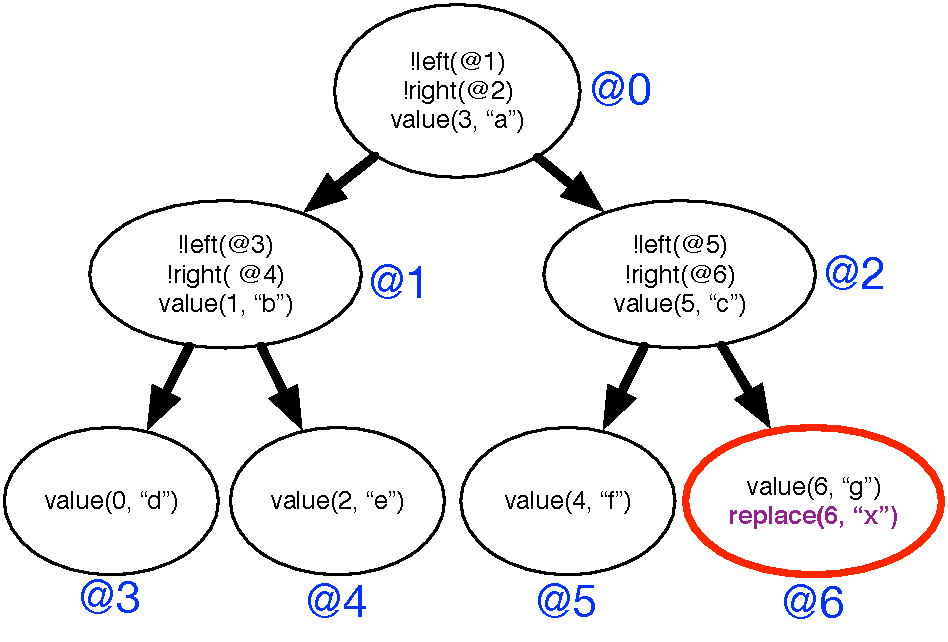
\includegraphics[width=\textwidth]{figures/btree/btree_trace3}
                \caption{After applying rule 3 at node \texttt{@5}. Replace fact
                   reaches node \texttt{@6}.}
                \label{fig:btree_trace3}
        \end{subfigure}%
        ~
        \begin{subfigure}[b]{0.5\textwidth}
                  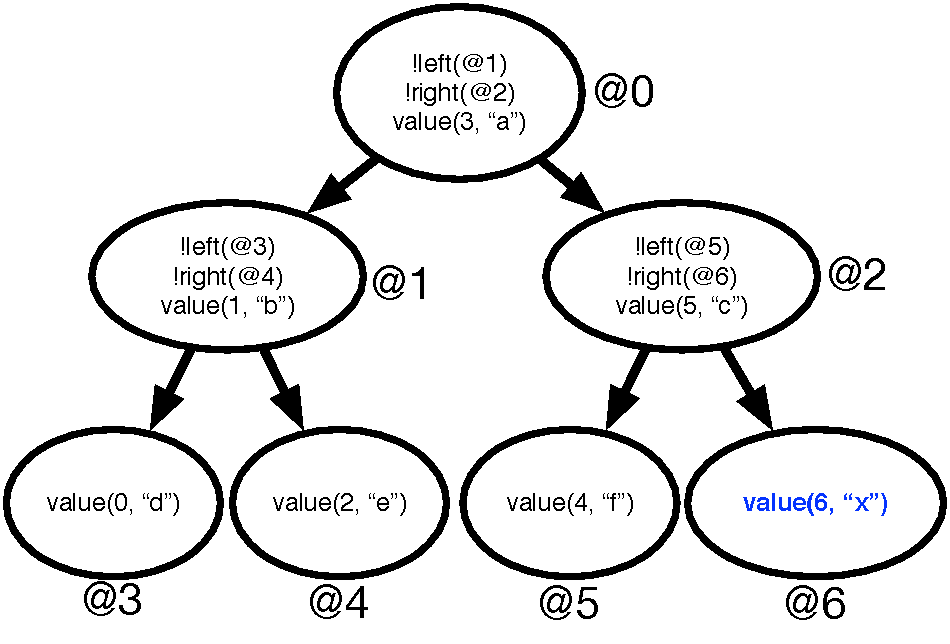
\includegraphics[width=\textwidth]{figures/btree/btree_trace4}
                  \caption{After applying rule 1 at node \texttt{@6}. Value of key 6 has changed to 7.}
                  \label{fig:btree_trace4}
          \end{subfigure}
        \caption{An execution trace for the binary tree dictionary
           algorithm. The first argument of each fact was dropped and the
           address of the node was placed beside it.}\label{fig:btree_trace}
\end{figure}

The present example offers many opportunies for concurrency. If we have multiple
\texttt{replace/3} facts on different nodes, we can perform multiple value
updates at the same time without introducing any kind of database inconsistency.



\subsection{Third Example: Graph Visit}

\begin{figure}[h!]
\begin{LineCode}[commandchars=\*\[\]]
type edge(node, node).*hfill// Predicate declaration
type linear visit(node).
type linear unvisited(node).
type linear visited(node).

visit(A), *label[line:language:visit_first1]*hfill // Rule 1: visit node
unvisited(A) -o
   visited(A),
   {B | !edge(A, B) -o visit(B)}.*label[line:language:visit_first2]*label[line:language:visit_comprehension]

visit(A),*label[line:language:visit_second1]*hfill // Rule 2: node already visited
visited(A)
   -o visited(A).*label[line:language:visit_second2]
\end{LineCode}
  \mycap{LM code for the graph visit program.}
  \label{code:language:visit}
\end{figure}

Our third example, shown in Fig.~\ref{code:language:visit}, presents another LM
program that, for a given graph of nodes, performs a visit to all nodes
reachable from node \code{@1}. The first rule of the program
(lines~\ref{line:language:visit_first1}-\ref{line:language:visit_first2}) visits
node \code{A} for the first time: fact \code{visited(A)} is derived and a
\emph{comprehension} construct is used to go through all the edge facts and then
derive \code{visit(B)} at each neighbor node \code{B}. The second rule of the
program
(lines~\ref{line:language:visit_second1}-\ref{line:language:visit_second2})
applies when the node is already visited more than once: we keep the
\code{visited} fact and delete \code{visit}. The initial facts shown in
Fig.~\ref{code:language:visit_initial} use the \code{visit(@1)} fact to start
the program.

\begin{figure}[h!]
\begin{LineCode}[commandchars=\*\[\]]
!edge(@1, @2).
!edge(@1, @4).
!edge(@2, @3).
!edge(@2, @4).
!edge(@2, @1).
!edge(@3, @2).
!edge(@4, @1).
!edge(@4, @2).

unvisited(@1).
unvisited(@2).
unvisited(@3).
unvisited(@4).

visit(@1).
\end{LineCode}
  \mycap{Initial facts for the graph visit program. Nodes reachable from node \code{@1} will be marked as \code{visited}.}
  \label{code:language:visit_initial}
\end{figure}

Fig.~\ref{fig:exec_trace} shows a possible execution trace for the visit
program. After applying the first rule at node \code{@1} we get the database in
Fig~\ref{fig:exec_trace}~(b).  Note that node \code{@1} is now visited and nodes
\code{@2} and \code{@4} now have a \code{visit} fact. At this point, we could
either apply rule 1 at node \code{@2} or at node \code{@4}.  For this specific
trace, we apply the rule at node \code{@2}, resulting in
Fig.~\ref{fig:exec_trace}~(c). Node \code{@4} now has two \code{visit} facts,
thus we can apply rule 1 followed by rule 2, therefore consuming both
\code{visit} facts and deriving \code{visited}. In addition, we can also apply
rule 1 at node \code{@3} to reach the state of Fig.~\ref{fig:exec_trace}~(d).

\begin{figure}[h]
        \centering
        \begin{subfigure}[b]{0.45\textwidth}
                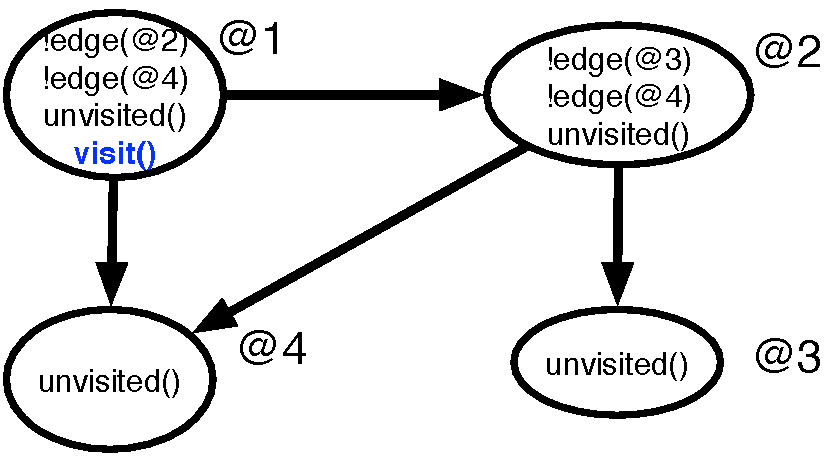
\includegraphics[width=\textwidth]{figures/visit/trace1}
                \mycap{Initial database.}
                \label{fig:exec_trace1}
        \end{subfigure}%
        ~ %add desired spacing between images, e. g. ~, \quad, \qquad etc.
          %(or a blank line to force the subfigure onto a new line)
        \begin{subfigure}[b]{0.45\textwidth}
                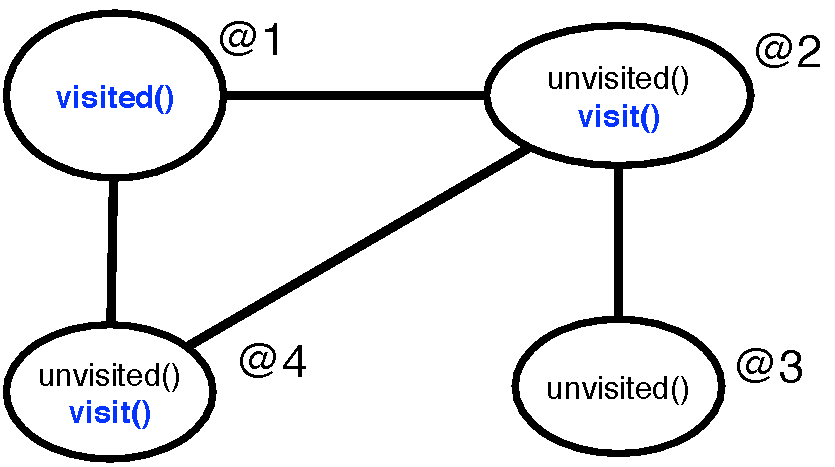
\includegraphics[width=\textwidth]{figures/visit/trace2}
                \mycap{After applying rule 1 at node \code{@1}.}
                \label{fig:exec_trace2}
        \end{subfigure}\\
        \begin{subfigure}[b]{0.45\textwidth}
                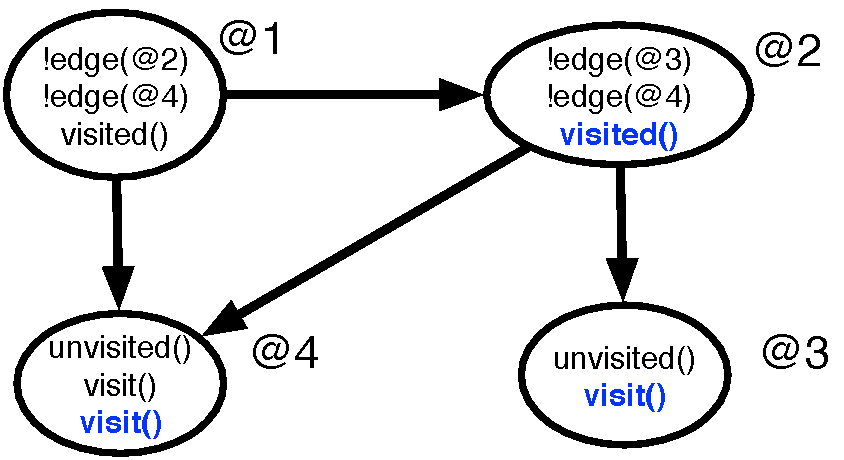
\includegraphics[width=\textwidth]{figures/visit/trace3}
                \mycap{After applying rule 1 at node \code{@2}.}
                \label{fig:exec_trace3}
        \end{subfigure}%
        ~ %add desired spacing between images, e. g. ~, \quad, \qquad etc.
         %(or a blank line to force the subfigure onto a new line)
        \begin{subfigure}[b]{0.45\textwidth}
                  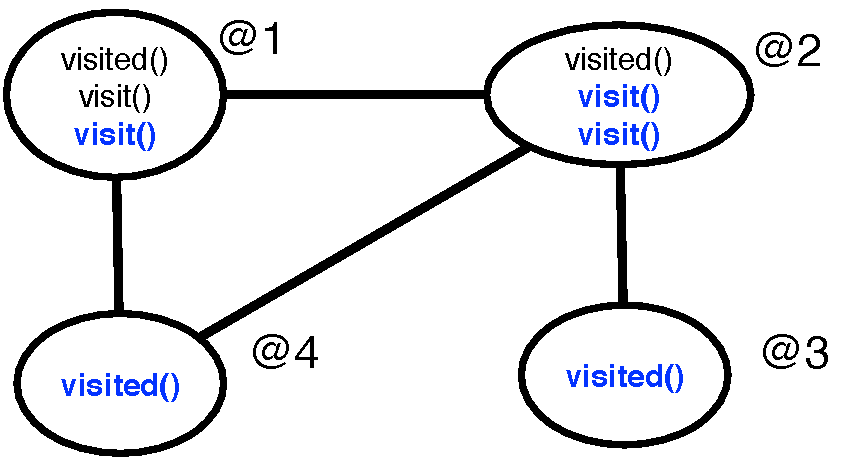
\includegraphics[width=\textwidth]{figures/visit/trace4}

                  \mycap{After applying rule 1 and 2 at node \code{@4} and
                  rule 1 at node \code{@3}.}

                  \label{fig:exec_trace4}
          \end{subfigure}
        \mycap{A possible execution trace for the visit
           program. Note that the \code{edge} facts were omitted for simplicity.}
        \label{fig:exec_trace}
\end{figure}

The graph visit has the potential to have plenty of concurrency. Once the visit
starts from the initial node, it expands to other nodes, allowing several nodes
to derive rules concurrently. At some point, the amount of concurrency is
reduced because more and more nodes have been visited. The level of concurrency
depends on the structure of the graph. In the worst case, if the graph is a
chain of nodes then the program becomes effectively sequential.  In the best
case, if the graph is densily connected (each node connects to most nodes in the
graph), then it is possible to run the program on most nodes at the same time.

The goal of introducing higher-level declarative languages is to facilitate
reasoning about the properties of a program. In the case of the visit program,
the most important goal is to prove that, if the graph is connected, then all
the nodes will become \code{visited}, regardless of the order in which we apply
the rules. First, we define a visit graph:

\begin{definition}[Visit graph]
A visit graph is an ordered pair $G = (N, E)$ comprising a set $N$ of nodes together
with a set $E$ of edges. Set $E$ contains pairs $(A, B)$ that correspond to
facts $\bang \mathtt{edge}(A, B)$. For every pair $(A, B) \in E$ there is also a
pair $(B, A) \in E$, representing an undirected edge.
\end{definition}

To prove the correctness property of the program, we first define the main
\emph{invariant} of the program:

\begin{invariant}[Node state]
A node is either \code{visited} or \code{unvisited} but not both.
\end{invariant}

\begin{proof}

From the initial facts we check if all nodes start as \code{unvisited}. This is
clearly true for the previous example. Rule 1 changes a node from
\code{unvisited} to \code{visited}, while rule 2 keeps the node \code{visited},
proving the invariant.

\end{proof}

Invariants are conditions that never change, no matter which rules are derived
during execution. With this invariant, it is now possible to classify nodes of
the graph $G$ according to their state:

\begin{definition}[Node sets] \code{visited} nodes are contained in set $V$,
while \code{unvisited} nodes are in set $U$. From the node state invariant, we
know that $V \cup U = N$ and $V \cap U = \emptyset$.
\end{definition}

We can now prove an important lemma about sets $V$ and $U$:

\begin{invariant}[Visited set]

After each rule derivation, visited set $V$ always increases or stays the same
size. The inverse is true for set $U$.

\end{invariant}
\begin{proof}
Initially, $V = \emptyset$ and $U = N$.
By rule 1, $V$ increases by 1 while $U$ decreases by 1. With rule 2, set
membership remains unchanged.
\end{proof}

In turn, since set membership changes from $U$ to $V$, we now prove the
following:

\noindent\begin{minipage}{\linewidth}
\begin{lemma}[Edge visits]\label{lemma:language:edge_visits}
The program generates at most one \code{visit} per directed edge and for a node
$a \in N$ that receives a \code{visit} fact, then for all $b \in N$ where $(a,
b) \in E$, exactly one \code{visit} fact is generated at $b$.
\end{lemma}
\end{minipage}
\begin{proof}
From the visited set invariant, we know that once nodes become members of set $V$,
they no longer return to set $U$, therefore rule 1 applies once per
node. This rule generates a \code{visit} fact per neighbor node.
\end{proof}

In order to prove that all the nodes in the graph are visited, we need to make
sure that the graph is connected.

\begin{definition}[Connected graph]
A connected graph is a graph where every pair of nodes has a path between them.
\end{definition}

Finally, we prove that all nodes will become \code{visited}.

\begin{theorem}[Graph visit correctness]
If graph $G$ is connected, set $V$ will eventually include all nodes in $N$,
while $U = \emptyset$.
\end{theorem}
\begin{proof}
Proof by induction.

\begin{itemize}

   \item Base case: initial fact \code{visit(@1)} adds node \code{@1} to $V$.
      By Lemma~\ref{lemma:language:edge_visits}, a \code{visit} fact is generate
      for all edges of \code{@1}.

   \item Inductive case: assume visited set $V'$ and unvisited set $U'$.
  Since the graph
   is connected, there must be a node $a \in V'$ that is connected to a node $b
   \in U'$. Using the Edge visits lemma, a $\mathtt{visit}(b)$ fact is generated,
   swapping $b$ from $U'$ to $V'$.
\end{itemize}

Eventually, set $V$ will include all nodes in $N$. Otherwise, there would be
unreachable nodes in the graph and that would be a contradiction since the graph
is connected.
\end{proof}



\section{Types and Locality}

Each fact is an association between a \emph{predicate} and a tuple of values. A
predicate is a pair with a name and a tuple of types (the argument types). LM
rules are type-checked using the predicate declarations in the header of the
program. LM has a simple type system that includes the following basic types:
\emph{node}, \emph{int}, \emph{float}, \emph{string}, \emph{bool}. The following
structured types are also supported: \emph{list} $X$, for lists of type $X$;
\emph{struct} $X_1, \ldots, X_n$, for composite values made of $n$ elements; and
\emph{array} $X$, for arrays of type $X$.

LM allows the definition of new type names from simpler types using the
declaration \code{type simple-type new-type} in the header of the program. The
type \code{new-type} can then be used as any other type. Note that LM uses
\emph{structural equivalence} to check if two types are the same, therefore
\code{simple-type} and \code{new-type} are type equivalent.

Type checking LM programs is straightforward due to its simple type system and
mandatory predicate declarations. For each rule, the variables found in the LHS
are mapped to types based on their use on atomic proposition arguments. Some
constraints of the form \code{X = expression} that force an equality between
\code{X} and \code{expression} may actually represent an \emph{assignment} if
\code{X} is not defined by any LHS atomic proposition. In this case, all the
variables in \code{expression} must be typed and \code{X} is assigned the value
of \code{expression} during run time.  Any variable used in the RHS of the rule
must be defined in the LHS, because otherwise derived facts would not be
\emph{grounded}, that is, some arguments would be undefined or uncomputable.
For comprehensions (and aggregates), type checking is identical, however, the LHS
of each construct must declare explicitly the variables in scope.

Another important component of type checking is \emph{locality checking}. The
first argument of each atomic proposition in the LHS must use the same variable
in order to enforce locality and allow concurrency. This \emph{home variable} is
always typed as a \emph{node} and represents a node in the graph. In the rule's
RHS, other home variables are allowed, as long as they have been defined in the
LHS. For comprehensions, the LHS must use the same home argument as the rule's
LHS.

\section{Operational Semantics}\label{sec:language:semantics}

Nodes are selected to computation non-deterministically (i.e., any node can be
picked to run). This means that the programmer cannot expect that facts coming
from different nodes will be considered as a whole since the process is
non-deterministic. The operational semantics promises that rule derivations are
performed atomically, therefore if a rule derives many facts belonging to a node
then that node will receive them all at once. Under these restrictions,
computation can then be parallelized by processing nodes concurrently.

Each rule in LM has a defined priority that is inferred from its position in the
source file. Rules at the beginning of the file have higher priority. At the
node level, we consider all the new facts that have not been considered yet to
create a queue of \emph{candidate rules}. The queue of candidate rules
is then applied (in priority order) and updated as new facts are derived or
consumed. As an example, consider the following three rules:

\begin{Code}
f(A), g(A) -o f(A).

h(A) -o g(A).

g(A) -o 1.
\end{Code}

If the database contains the facts \code{h(@1)} and \code{f(@1)}, then the
second rule is applied, retracting \code{h(@1)} and deriving \code{g(@1)}. Next,
the first and third rules are candidate rules, but since the first rule has
higher priority, it is applied first, resulting in a database with a single fact
\code{f(@1)}, where no rule can be applied. Later, in
Section~\ref{sec:implementation:rule_engine}, we give more details about how our
implementation manages the set of candidate rules.



\section{LM Abstract Syntax}
Table~\ref{tbl:language:ast} shows the abstract syntax for rules in LM.  A LM
program $Prog$ consists of a list of derivation rules $\Sigma$ and a database
$D$. A database fact $l(\hat{t})$ is an association between a predicate $l$ and
a list of literals $\hat{t}$. Each derivation rule $R$ can be written as $LHS
\lolli RHS$ with the meaning described in
Section~\ref{section:language:message}.  Rules without an LHS are allowed in LM
and they are called \emph{initial facts}
(lines~\ref{line:language:dict_axioms1}-\ref{line:language:dict_axioms2} in
Fig.~\ref{code:language:btree_replace}).

\newcommand{\sop}[0]{\Vert}

\begin{table}[h]
\centering
\begin{tabular}{ l l c l }
  Program & $Prog$ & $::=$ & $\Sigma, D$ \\
  List Of Rules & $\Sigma$ & $::=$ & $\cdot \; \sop \; \Sigma, R$\\
  Database & $D$ & $::=$ & $\Gamma; \Delta$ \\
  Rule & $R$ & $::=$ & $LHS \lolli RHS \; \sop \; \forall_{x}. R \; \sop \;
  \selector{S}{y}{LHS}{RHS}$ \\
  LHS Expression & $LHS$ & $::=$ & $L \; \sop \; P \; \sop \; C \; \sop \; LHS,
  LHS \; \sop \; \exists_{x}. LHS \; \sop \; \one$\\
  RHS Expression & $RHS$ & $::=$ & $L \; \sop \; P \; \sop \; RHS, RHS \; \sop
  \; EE \; \sop \; CE \; \sop \; AE \; \sop \; \one$\\
  
  Linear Atomic Proposition & $L$ & $::=$ & $l(\hat{x})$\\
  Persistent Atomic Prop. & $P$ & $::=$ & $\bang p(\hat{x})$\\
  Constraint & $C$ & $::=$ & $c(\hat{x})$ \\
  Selector Operation & $S$ & $::=$ & $\mathtt{min} \; \sop \; \mathtt{max} \;
  \sop \; \mathtt{random}$\\
  
  Exists Expression & $EE$ & $::=$ & $\existsc{\widehat{x}}{SRHS}$ \\
  Comprehension & $CE$ & $::=$ & $\comprehension{\widehat{x}}{SLHS}{SRHS}$ \\

  Aggregate & $AE$ & $::=$ & $\aggregate{A}{y}{\widehat{x}}{SLHS}{SRHS_1}{SRHS_2}$ \\
  Aggregate Operation & $A$ & $::=$ & $\mathtt{min} \; \sop \; \mathtt{max} \; \sop \;
\mathtt{sum} \; \sop \; \mathtt{count} \; \sop \; \mathtt{collect}$ \\
  
  Sub-LHS & $SLHS$ & $::=$ & $L \; \sop \; P \; \sop \; SLHS, SLHS \; \sop \; \exists_{x}. SLHS$\\
  Sub-RHS & $SRHS$ & $::=$ & $L \; \sop \; P \; \sop \; SRHS, SRHS \; \sop \; \one$\\
  
  Known Linear Facts & $\Delta$ & $::=$ & $\cdot \; \sop \; \Delta, l(\hat{t})$ \\
  Known Persistent Facts & $\Gamma$ & $::=$ & $\cdot \; \sop \; \Gamma, \bang p(\hat{t})$ \\

  Literal List & $\hat{t}$ & $::=$ & $\cdot \; \sop \; t, \hat{t}$ \\
  Term List & $\hat{x}$ & $::=$ & $\cdot \; \sop \; x, \hat{x} \; \sop \; t, \hat{x}$ \\
  Literal & $t$ & $::=$ & $\m{number}(N) \; \sop \; \m{node}(N) \; \sop \; \m{list}(\hat{t}) \; \sop \ldots$ \\
\end{tabular}
\caption{Core abstract syntax of LM.}\label{tbl:language:ast}
\end{table}

The LHS of a rule, $LHS$, may contain linear ($L$) and persistent ($P$)
\emph{atomic propositions} and constraints ($C$). Atomic propositions are
template facts that instantiate variables (from facts in the database) such as
\code{visit(A)} in line~\ref{line:language:visit_second} in
Fig.~\ref{code:language:visit}. Variables can be used again in the LHS for
matching and also in the RHS when instantiating facts.  Constraints are boolean
expressions that must be true in order for the rule to be derived. Constraints
use variables from fact expressions and are built using a small functional
language that includes mathematical operations, boolean operations, external
functions and literal values.

The RHS of a rule, $RHS$, contains linear ($L$) and persistent ($P$)
\emph{atomic propositions} which are uninstantiated facts. The RHS can also have
\emph{exists expressions} ($EE$), \emph{comprehensions} ($CE$) and
\emph{aggregates} ($AE$). All those expressions may use all the variables
instantiated in the rule's LHS and are explained in detail in
Section~\ref{section:language:expressions}.

\subsubsection{Graph visit using the abstract syntax}\label{visit:ast}

Consider the two rules in the graph visit program shown in
Fig.~\ref{code:language:visit}:

\nopagebreak

\begin{Verbatim}[fontsize=\codesize]
visit(A), unvisited(A) -o visited(A), {B | !edge(A, B) -o visit(B)}.

visit(A), visited(A) -o visited(A).
\end{Verbatim}

To translate the rules to the abstract syntax, we have to de-sugar the code and
introduce the variable \code{A}, that is not explicitly quantified, as follows:

\nopagebreak

\begin{align}
\forall_A. \mathtt{visit}(A), \; \mathtt{unvisited}(A) \lolli & \;
\mathtt{visited}(A), \; \comprehension{B}{\mathtt{edge}(A, B)}{\mathtt{visit}(B)}\\
\forall_A. \mathtt{visit}(A), \; \mathtt{visited}(A) \lolli & \;
\mathtt{visited}(A)
\end{align}

Finally, initial facts are represented as a rule where the LHS is $\one$:

\nopagebreak

\begin{align}
\one \lolli & \bang \mathtt{edge}(@1, @2) \\
\one \lolli & \bang \mathtt{edge}(@2, @3) \\
\one \lolli & \bang \mathtt{edge}(@1, @4) \\
\one \lolli & \bang \mathtt{edge}(@2, @4) \\
\one \lolli & \mathtt{unvisited}(@1)  \\
\one \lolli & \mathtt{unvisited}(@2) \\
\one \lolli & \mathtt{unvisited}(@3) \\
\one \lolli & \mathtt{unvisited}(@4) \\
\one \lolli & \mathtt{visit}(@1)
\end{align}

\subsection{RHS Expressions}\label{section:language:expressions}

\subsubsection{Selectors}

When a rule's LHS is instantiated using facts from the database, facts are
picked non-deterministically. While our system uses an implementation dependent
order for efficiency reasons, sometimes it is important to sort facts by one of
the arguments. The abstract syntax for this construct is
$\selector{S}{y}{LHS}{RHS}$, where $S$ is the selection operation and $y$ is the
variable in $LHS$ that represents the value to be selected according to $S$. An
example using concrete syntax is as follows:

\begin{Verbatim}[fontsize=\codesize]
[min => W | !edge(A, B), weight(A, B, W)] -o picked(A, B, W).
\end{Verbatim}

In this case, we order the \code{weight} facts by \code{W} in ascending order
and then try to match them. Other operations available are \code{max} and
\code{random} (to force no pre-defined order at the implementation level).

\subsubsection{Exists Expression}

Exists constructs ($EE$) are based on the linear logic construct of the same name
and are used to create fresh node addresses. We can use the new address to
instantiate new facts for the new node. As an example, consider the implementation of the
insertion operation for the key/value dictionary described in
Fig.~\ref{code:language:btree_replace}:

\begin{Verbatim}[fontsize=\codesize]
insert(A, IKey, IValue),
value(A, Key, Value),
IKey < Key
   -o value(A, Key, Value),
      exists B. (value(B, IKey, IValue), !left(A, B)).
\end{Verbatim}

The exists construct is used to create the left node of node \code{A} that
contains \code{value(B, IKey, IValue)} (the newly inserted key/value pair) and
the persistent fact \code{!left(A, B)} that connects \code{A} to \code{B}.

\subsubsection{Comprehensions}

Sometimes we need to consume a linear fact and then immediately generate several
facts depending on the contents of the database. To solve this particular need,
we created the concept of comprehensions, which are sub-rules that are applied
with all possible combinations of facts from the database. In a comprehension
$\comprehension{\widehat{x}}{SLHS}{SRHS}$, $\widehat{x}$ is a list of variables
in the scope of $SLHS$ and $SRHS$, $SLHS$ is the comprehension's left-hand side
and $SRHS$ is the right-hand side. $SLHS$ is used to generate all possible
combinations for $SRHS$, according to the facts in the database. We have already
seen an example of comprehensions in the visit program
(Fig.~\ref{code:language:visit} line~\ref{line:language:visit_comprehension}):

\begin{Verbatim}[fontsize=\codesize,commandchars=\*\#\&]
visit(A), unvisited(A) -o visited(A), *textbf#{B | !edge(A, B) -o visit(B)}&.
\end{Verbatim}

We match \code{!edge(A, B)} using all the combinations available in the database
and for each combination we derive \code{visit(B)}.

\subsubsection{Aggregates}

Another useful feature in logic programs is the ability to reduce several facts
into a single fact. LM features aggregates ($AE$), a special kind of sub-rule
that works somewhat like comprehensions. In the abstract syntax
$\aggregate{A}{y}{\widehat{x}}{SLHS}{SRHS_1}{SRHS_2}$, $A$ is the aggregate
operation, $\widehat{x}$ is the list of variables introduced in $SLHS$, $SRHS_1$
and $SRHS_2$ and $y$ is the variable in $SLHS$ that represents the values to be
aggregated using $A$. Like comprehensions, we use $\widehat{x}$ to try all the
combinations of $SLHS$, but, in addition to deriving $SRHS_1$ for each
combination, we aggregate the values represented by $y$ into a new $y$ variable
that is used to derive $SRHS_2$.

To better understand aggregates, let's consider the following rule from the
PageRank program presented in Section~\ref{section:language:pagerank}:

\begin{Verbatim}[fontsize=\codesize]
update(A),
!numInbound(A, T)
   -o [sum => V; B, W, Val, Iter | neighbor-pagerank(A, B, Val, Iter), V =
         Val/float(T) -o neighbor-pagerank(A, B, Val, Iter) -> sum-ranks(A, V)].
\end{Verbatim}

The rule aggregates the PageRank values \code{Val} by iterating over
\code{neighbor-pagerank(A, B, Val, Iter)} (the $SLHS$) and then re-deriving the
fact present in $SRHS_1$ using \code{neighbor-pagerank(A, B, Val, Iter)}. Once all
values are inspected, the atomic proposition \code{sum-ranks(A, V)} present in
$SRHS_2$ is derived once with \code{V} that represents the sum of all the
neighbor values. LM provides several aggregate operations, including the
\code{min} (minimum value), \code{max} (maximum value), \code{sum} (add all
numbers), \code{count} (count combinations) and \code{collect} (collect items
into a list).

\section{Types and Locality}

Each fact is an association between a \emph{predicate} and a tuple of values. A
predicate is a pair with a name and a tuple of types (the argument types). LM
rules are type-checked using the predicate declarations in the header of the
program. LM has a simple type system that includes the following simples types:
\emph{node}, \emph{int}, \emph{float}, \emph{string}, \emph{bool}. The following
structured types are also supported: \emph{list} $X$, for lists of type $X$;
\emph{struct} $X_1, \ldots, X_n$, for composite values made of $n$ elements; and
\emph{array} $X$, for arrays of type $X$.

LM allows definition of new type names from simpler types using the declaration
\code{type simple-type new-type} in the header of the program. The type
\code{new-type} can then be used as any other type. Note that LM uses
\emph{structural equivalence} to check if two types are the same, therefore
\code{simple-type} and \code{new-type} are type equivalent.

Type checking LM programs is straightforward due to its simple type system and
mandatory predicate declarations. For each rule, the variables found in the LHS
are mapped to types based on their use on atomic proposition arguments. Some
constraints of the form \code{X = expression} that force an equality between
\code{X} and \code{expression} may actually represent an assignment of
\code{expression} to a variable \code{X} since \code{X} may not be used in any
proposition argument. In this case, all the variables in \code{expression} must
be typed or else \code{X} becomes an \emph{undefined variable}. Variables in the
rule's RHS must be defined in the LHS, because otherwise derived facts would not
be \emph{ground}, that is, some arguments would be undefined or uncomputable.
For the comprehensions and aggregates, the type checking rules are identical,
however the LHS of each construct must document the variables in scope using the
$\hat{x}$ argument. If a variable is introduced in the LHS that is not in
$\hat{x}$, type checking will fail.

Another important part of type checking is \emph{locality checking}. The first
argument of each atomic proposition in the LHS must use the same variable in
order to enforce locality and allow concurrency. This \emph{home variable} is
always typed as a \emph{node} and represents a node in the program's graph. In
the rule's RHS, other home variables are allowed, as long as they are defined
variables. For comprehensions and aggregates, the LHS must use the same home
argument as the rule's LHS.

\section{Operational Semantics}

As said before, the first argument of every predicate must be typed as a
\emph{node}.  For distribution purposes, the LHS of all rules can only use facts
from the same node in order to make concurrency possible. However, the facts in
the rule's RHS may refer to other nodes, as long as those nodes are instantiated
in the LHS. We drew some inspiration from the Linda system~\cite{linda}
mentioned early on, where the tuple space contains the data and is used by the
processors to communicate and perform computation. This differs from imperative
languages, since in those languages data and computation are two separate
entities.

The execution is performed at the node level and happens non-deterministically
(i.e., any node can be picked to run). This means that the programmer cannot
expect that facts coming from different nodes will be considered as a whole or
partially since the process is non-deterministic. The operational semantics
promises that rule derivations are performed atomically, therefore if a rule
sends many facts to a node then the target node will receive them all at once.
Under these restrictions, computation can then be parallelized by processing
many nodes concurrently.

Each rule in LM has a defined priority that is inferred from its position in the
source file.  Rules at the beginning of the file have higher priority. At the
node level, we consider all the new facts that have not been considered before
to create a priority queue of \emph{candidate rules}. The queue of candidate
rules is then applied (by priority) and updated as new facts are derived or
consumed. As an example, consider the following three rules:

\begin{Verbatim}[fontsize=\codesize]
f(A), g(A) -o f(A).

h(A) -o g(A).

g(A) -o 1.
\end{Verbatim}

If the database contains the facts \code{h(@1)} and \code{f(@1)}, then the
second rule is applied, deriving \code{g(@1)} and retracting \code{h(@1)}. Next,
the first and third rules are candidate rules, but since the first rule has
higher priority, it is applied immediately, resulting in a database with a
single fact \code{f(@1)}.  Section~\ref{sec:implementation:rule_engine} gives
details in how our implementation manages the set of candidate rules.


\section{Applications}
In this section, we present solutions to well-known problems. We start with
straightforward graph-based problems such as bipartitness checking and two
versions of the PageRank program. Next, we present the LM version of the
Quick-Sort algorithm, which from a first impression may not fit well under the
programming paradigm offered by LM. Informal correctness and termination proofs
are also included to further show that such important properties are relatively
easy to prove for programs written in LM.

\subsection{Bipartiteness Checking}

The problem of checking if a graph is bipartite can be seen as a 2-color graph
coloring problem.  The code for this algorithm is shown in
Fig.~\ref{language:code:bichecking}. All nodes in the graph start as
\texttt{uncolored}, because they do not have a color yet. The axiom
\texttt{visit(@1, 1)} is instantiated at node \texttt{@1}
(line~\ref{line:language:bc_axiom}) in order to color it with color 1.

If a node is \texttt{uncolored} and needs to be marked with a color \texttt{P}
then the rule in
lines~\ref{line:language:bc_first1}-\ref{line:language:bc_first2} is applied. We
consume the \texttt{uncolored} fact and derive a \texttt{colored(A, P)} to
effectively color the node with \texttt{P}. We also derive \texttt{visit(B,
next(P))} in neighbor nodes to color them with the other color. 

The coloring can fail if a node is already colored with a color \texttt{P} and
needs to be colored with a different color (line~\ref{line:language:bc_third})
or if it has already failed (line~\ref{line:language:bc_fourth}).

\begin{figure}[h!]
\begin{Verbatim}[numbers=left,fontsize=\codesize,commandchars=\*\[\]]
type route edge(node, node).
type linear visit(node, int).
type linear uncolored(node).
type linear colored(node, int).
type linear fail(node).

fun next(int X) : int = if X <> 1 then 1 else 2 end.

visit(@1, 1).*label[line:language:bc_axiom]

visit(A, P), uncolored(A)*label[line:language:bc_first1]
   -o {B | !edge(A, B) | visit(B, next(P))},
      colored(A, P).*label[line:language:bc_first2]

visit(A, P), colored(A, P) -o colored(A, P).*label[line:language:bc_second]
visit(A, P1), colored(A, P2), P1 <> P2 -o fail(A).*label[line:language:bc_third]
visit(A, P), fail(A) -o fail(A).*label[line:language:bc_fourth]
\end{Verbatim}
  \caption{Bipartiteness Checking program.}
  \label{language:code:bichecking}
\end{figure}

\subsubsection{Proof Of Correctness}

In order to show that the code in Fig.~\ref{language:code:bichecking} works as
intended, we first setup some invariants that hold throughout the execution of
the program. Assume that the set of nodes in the graph is represented as $N$.

\begin{invariant}[Node state]
Set of nodes $N$ is partitioned into 4 different states that represent the 4
possible states that a node can be in, namely:

\begin{itemize}
   \item $U$ (\texttt{uncolored} nodes)
   \item $F$ (\texttt{fail} nodes)
   \item $C_{true}$ (\texttt{colored(A, 1)} nodes)
   \item $C_{false}$ (\texttt{colored(A, 2)} nodes)
\end{itemize}
\end{invariant}
\begin{proof}
Initially, all nodes start in set $U$. All the 4 rules of the programs either
keep the node in the same set or exchange the node with another set.
\end{proof}

A bipartite graph is one where in every edge $a \leftrightarrow b$, there is a
valid assignment that makes $a$ member of set $C_{true}$ or $C_{false}$ and node
$b$ member of either $C_{false}$ or $C_{true}$ respectively.

\begin{lemma}[Bipartiteness
   Convergence]\label{language:lemma:bipartite_convergence}
   We now reason from the application of the program rules. After each
   application of an inference rule, one of the following will happen:

   \begin{itemize}
      \item Set $U$ will decrease and set $C_{true}$ or $C_{false}$ will
         increase, with a potential increase in the number of \texttt{visit}
         facts.
      \item Set $C_{true}$ or $C_{false}$ will stay the same, while the number
         of \texttt{visit} facts will be reduced.

      \item Set $C_{true}$ or $C_{false}$ will decrease and set $F$ will
         increase, while the number of \texttt{visit} facts will be reduced.

      \item Set $F$ will stay the same, while the number of \texttt{visit} facts
         decreases.
   \end{itemize}

\end{lemma}
\begin{proof}
Directly from the rules.
\end{proof}

From this invariant, it can be inferred that set $U$ never increases in size
and in a node transition from \texttt{uncolored} to \texttt{colored}, the
database may increase in size. For every other rule application, the database of
facts always decreases. This also means that the program will eventually
terminate, since it is limited by the number of \texttt{visit} facts that can be
generated.

\begin{theorem}[Bipartiteness Correctness]
If the graph is connected and bipartite then the nodes will be partitioned into
sets $C_{true}$ and $C_{false}$, while sets $F$ and $U$ are empty.
\end{theorem}
\begin{proof}
   By induction, we prove that uncolored nodes become part of either $C_{true}$
   and $C_{false}$ and, if there is an edge between nodes in the two sets then
   they have different colors.

   In the base case, we start with empty sets but node \texttt{@1} is made
   member of $C_{true}$. Rule 1 sends \texttt{visit} facts to the neighbors of
   \texttt{@1}, forcing them to be members of $C_{false}$.

   In the inductive case, we have sets $C'_{true}$ and $C'_{false}$ with some
   nodes already colored. From Lemma~\ref{language:lemma:bipartite_convergence},
   we know that $U$ always decreases. Since the graph is bipartite, events 3 and
   4 never happen since there is a possible partitioning of nodes. With event 1,
   we have set $C_{true} = C'_{true}, n$, (or $C_{false}$) where $n$ is the
   node and with event 2, the sets remain the same. Since the graph is
   connected, every node will be colored, therefore event 1 will happen for
   every node of the graph.
\end{proof}

\subsection{PageRank}

PageRank~\cite{Page:2001:MNR} is a well known graph algorithm that is used to
compute the relative relevance of web pages.  The code for a synchronous version
of the algorithm is shown in Fig.~\ref{language:code:pagerank}. As the name
indicates, the pagerank is computed for a certain number of iterations. The
initial pagerank is the same for every page and is initialized in the first rule
(lines
\ref{line:language:spagerank_first1}-\ref{line:language:spagerank_first2}) along
with an accumulator.

The second rule of the program
(lines~\ref{line:language:spagerank_second1}-\ref{line:language:spagerank_second2})
propagates a newly computed pagerank value to all neighbors. The fact
\texttt{neighbor-pagerank} informs the neighbor node about the pagerank value of
node \texttt{A} for iteration \texttt{Iter + 1}. For every iteration, each node
will accumulate the all the \texttt{neighbor-pagerank} facts into the
\texttt{accumulator} fact (lines
\ref{line:language:spagerank_fourth1}-\ref{line:language:spagerank_fourth2}).
When all inbound neighbor pagerank values are accumulated, the third rule
(lines~\ref{line:language:spagerank_third1}-\ref{line:language:spagerank_third2})
is fired and a pagerank value is derived for iteration \texttt{Iter}.

\begin{figure}[h!]
\begin{Verbatim}[numbers=left,fontsize=\codesize,commandchars=\*\[\]]
type outbound(node, node, float).
type linear pagerank(node, float, int).
type numInbound(node, int).
type linear accumulator(node, float Acc, int Left, int Iteration).
type linear neighbor-pagerank(node, node Neighbor, float Rank, int Iteration).
type linear start(node).

const damping = 0.85. // probability of user following a link in the current page.
const iterations = str2int(@arg1). // iterations to compute.
const pages = @world. // number of pages in the graph.

start(A).

start(A), !numInbound(A, T)*label[line:language:spagerank_first1]
   -o accumulator(A, 0.0, T, 1), pagerank(A, 1.0 / float(pages), 0).*label[line:language:spagerank_first2]

pagerank(A, V, Iter), // propagate new pagerank value*label[line:language:spagerank_second1]
Iter < iterations
   -o {B, W | !outbound(A, B, W) | neighbor-pagerank(B, A, V * W, Iter + 1)}.*label[line:language:spagerank_second2]

accumulator(A, Acc, 0, Iter), // new pagerank*label[line:language:spagerank_third1]
!numInbound(A, T),
V = damping + (1.0 - damping) * Acc,
Iter <= iterations
   -o pagerank(A, V, Iter), accumulator(A, 0.0, T, Iter + 1).*label[line:language:spagerank_third2]
	
neighbor-pagerank(A, B, V, Iter), accumulator(A, Acc, T, Iter)*label[line:language:spagerank_fourth1]
   -o accumulator(A, Acc + V, T - 1, Iter).*label[line:language:spagerank_fourth2]
\end{Verbatim}
\caption{Synchronous PageRank program.}
\label{language:code:pagerank}
\end{figure}

\subsubsection{Asynchronous PageRank}

We also have an asynchronous version of the algorithm that trades correctness
with convergence speed since it does not synchronize between iterations.
Figure~\ref{language:code:async_pagerank} shows the LM code for this particular
version, where two major differences can be observed: (1) there is a linear fact
\texttt{neighbor-pagerank} containing the most up-to-date pagerank value of a
neighbor node; (2) a new \texttt{update} fact that forces the node to re-compute
its pagerank by processing the currently available \texttt{neighbor-pagerank}
facts. Rules in
lines~\ref{line:language:apagerank_update1}-\ref{line:language:apagerank_update2}
update the \texttt{neighbor-pagerank} values, while rule in
lines~\ref{line:language:apagerank_new1}-\ref{line:language:apagerank_new2}
asynchronously update the current pagerank value. This last rule derives
multiple \texttt{new-neighbor-rank} that is used to inform the neighbor about
the new pagerank value.

\begin{figure}[h!]
\begin{Verbatim}[numbers=left,fontsize=\codesize,commandchars=\*\#\&]
type outbound(node, node, float).
type linear pagerank(node, float, int).
type numInbound(node, int).
type linear neighbor-pagerank(node, node Neighbor, float Rank, int Iteration).
type linear new-neighbor-rank(node, node Neighbor, float Rank, int Iteration).
type linear update(A).
type linear sum-ranks(node, float).

pagerank(A, 1.0 / float(pages), 0).
update(A).
neighbor-pagerank(A, B, 1.0 / float(pages), 0). // pagerank of B is ...

// save incoming pagerank value.*label#line:language:apagerank_update1&
new-neighbor-rank(A, B, New, Iteration),
neighbor-pagerank(A, B, Old, OldIteration),
Iteration > OldIteration
   -o neighbor-pagerank(A, B, New, Iteration).
new-neighbor-rank(A, B, New, Iteration),
neighbor-pagerank(A, B, Old, OldIteration),
Iteration <= OldIteration
   -o neighbor-pagerank(A, B, Old, OldIteration).*label#line:language:apagerank_update2&

sum-ranks(A, Acc),
NewRank = damping/float(pages) + (1.0 - damping) * Acc,
pagerank(A, OldRank, Iteration)
      -o pagerank(A, NewRank, Iteration + 1),
         {B, W, Delta, Iter | !outbound(A, B, W), Delta = fabs(NewRank -
               OldRank) * W | new-neighbor-rank(B, A, NewRank, Iteration + 1),
               if Delta > bound then update(B) end}.

update(A), update(A) -o update(A).

update(A),*label#line:language:apagerank_new1&
!numInbound(A, T)
   -o [sum => V | B, W, Val, Iter | neighbor-pagerank(A, B, Val, Iter),
         V = Val/float(T) | neighbor-pagerank(A, B, Val, Iter) | sum-ranks(A, V)].*label#line:language:apagerank_new2&
\end{Verbatim}
\caption{Asynchronous PageRank program.}
\label{language:code:async_pagerank}
\end{figure}

\subsubsection{Proof Of Correctness}

To build the proof of correctness, we must again prove several program
invariants. This will help us prove that this partifcular program is similar to
a computation on a nonnegative matrix of of unit spectral radius, which has been
proven that it converges~\cite{DBLP:journals/corr/abs-cs-0606047,
Lubachevsky:1986:CAA:4904.4801}.

\begin{invariant}[Page Invariant]
Each page/node has a single \texttt{pagerank(A, Value, Iteration)} and:
\begin{itemize}
   \item For each outbound link, a single \texttt{\bang outbound(A, B, W)}.
   \item For each inbound link, a single \texttt{neighbor-pagerank(A, B, V, Iter)}.
   \item For each \texttt{\bang outbound(A, B, W)}, a \texttt{neighbor-pagerank(A,
      B, V, Iter}.
\end{itemize}
\end{invariant}

\begin{proof}

All axioms validate the 3 conditions of the variant. Note that the third
condition is also validated by the axioms, although not all axioms are shown in
the code.

In relation to rule application:

\begin{itemize}
   \item Rule 1: inbound link re-derived.
   \item Rule 2: inbound link re-derived.
   \item Rule 3: \texttt{pagerank/2} re-derived.
   \item Rule 4: Nothing happens.
   \item Rule 5: inbound links re-derived in the comprehension.
\end{itemize}
\end{proof}

\begin{lemma}[Neighbor rank lemma]
Given a fact \texttt{neighbor-pagerank(A, B, V, Iter)} and a set of facts
\texttt{new-neighbor-rank(A, B, New, Iter2)}, we end up with a single
\texttt{neighbor-pagerank(A, B, V', Iter')}, where \texttt{Iter} is the greater of
\texttt{Iter} or all of \texttt{Iter2'}.
\end{lemma}
\begin{proof}
By induction on the number of \texttt{new-neighbor-rank} facts.

Base case: \texttt{neighbor-pagerank} remains.

Inductive case: given one \texttt{new-neighbor-rank} fact:

\begin{itemize}
   \item Rule 1: the new iteration is older and thus \texttt{neighbor-pagerank}
   is replaced. By applying induction, we know that we will select either the
   new best iteration or a better iteration from the remaining set of
   \texttt{new-neighbor-rank} facts.
   \item Rule 2: the new iteration is not older and we keep the old
   \texttt{neighbor-pagerank} fact. By induction, we select the best from either
   the current iteration or some other (from the set).
\end{itemize}
\end{proof}

\begin{lemma}[Update lemma]
Given at least 1 \texttt{update/1} fact, rule 7 will run.
\end{lemma}
\begin{proof}
By induction on the number of \texttt{update} facts.

Base case: rule 5 will run.

Inductive case: rule 4 will run first because it has a higher priority, reducing
the number of \texttt{update} facts by one. By induction, we know that by
using the remaining \texttt{update} facts, rule 7 will run.
\end{proof}

\begin{lemma}[Pagerank update lemma]
(1) Given at least one \texttt{update} fact, the \texttt{pagerank(A, $V_{I}$,
I)} fact will be updated to become \texttt{pagerank(A, $V_{I + 1}$, I +
1)}, where \texttt{$V_{I + 1} = damping / P + (1.0 - damping)\sum_{B,
I} (W_{B} \times  N_{I,B})$}.

where $W_B = 1.0/T$ ($T$ from \texttt{\bang numInbound(A, $T$)})
and $N_{I,B}$ from \texttt{neighbor-pagerank(A, B, $N_{I, B}$, $I$)}.

(2) For all \texttt{B} outbound nodes (represented using \texttt{\bang outbound(A, B,
W)}, a \texttt{new-neighbor-rank(B, A, $V_{I+1}$, $I + 1$)} is generated.

(3) For all \texttt{B} outbound nodes (represented using \texttt{\bang outbound(A, B,
W)}), a \texttt{update(B)} is generated if 
$fabs(V_{I + 1} - V_{I}) \times W > bound$.
\end{lemma}
\begin{proof}
Using the Update lemma, rule 5 will necessarily run.

It derives \texttt{sum-ranks(A, $\sum_{B, I} (W_B \times N_{I,B})$)} and
fulfills (3).

\texttt{sum-ranks/2} will necessarily fire rule 6,
computing $V_{I+1}$ and updating \texttt{pagerank}. (2) and (3) are fulfilled
through the comprehension of rule 6.
\end{proof}

\begin{invariant}[New neighbor rank equality]
All \texttt{new-neighbor-rank(A, B, V, I)} facts are generated from a corresponding
\texttt{pagerank(B, V, I)} fact, therefore the iteration of any
\texttt{new-neighbor-rank} is at least the same or less than the iteration of
the current pagerank.
\end{invariant}
\begin{proof}
No axioms to prove.

\begin{itemize}
   \item Rule 3: true, new fact is generated.
   \item Rule 6: the fact is kept.
\end{itemize}
\end{proof}

\begin{invariant}[Neighbor rank equality]
All \texttt{neighbor-pagerank(A, B, V, I)} facts have one corresponding
\texttt{pagerank(B, V, I)} fact and the iteration of the \texttt{neighbor-pagerank}
is the same or less than the current iteration of the corresponding
\texttt{pagerank}.
\end{invariant}
\begin{proof}
By analyzing axioms and rules.

Axioms: true.

Rule cases:

\begin{itemize}
   \item Rule 1: uses \texttt{new-neighbor-rank} fact (use new neighbor rank
         equality invariant).
   \item Rule 2: same fact is re-derived.
\end{itemize}
\end{proof}

\begin{theorem}[Pagerank convergence]
The program will compute the pagerank of all nodes that is within \texttt{bound} error
of an asynchronous pagerank computation.
\end{theorem}
\begin{proof}

Using the program axioms, we start with the same pagerank value for all nodes.
The \texttt{\bang outbound(A, B, W)} fact forms a $n \times n$ square matrix (number
of nodes) and is the so-called "Google Matrix".  All the initial pagerank values
can be seen as a vector that adds up to $1$.

The pagerank computation from the "Pagerank update lemma" computes $V_{I + 1} =
damping / P + (1.0 - damping)\sum_{B, I'} (W_{B} \times N_{I',B})$, where $I' <=
I$
(from Neighbor rank equality invariant).

Consider that each node contains a column $G_i$ of the Google matrix. The
pagerank computation can then be represented as: \newline


$V_{I + 1} = G_i fix([N_{I_1, B_1}, ..., N_{I_p, B_p}])$ \hfill (1) \\


Where $p$ is the number of inbound links and $N_{I_j, B_j}$ is the value of
the \texttt{neighbor-pagerank(A, $B_j$, $N_{I_j, B_j}$, $I_j$)}. The $fix()$
function takes the neighbor vector and expands it with zeros corresponding to
nodes that are not inbound links.

From~\cite{DBLP:journals/corr/abs-cs-0606047, Lubachevsky:1986:CAA:4904.4801} we
know that equation (1) will improve (converge) the pagerank value, given that some new
neighbor pagerank values are sent to node $i$ and by the fact that $G_i$ is a
nonnegative matrix of unit spectral radius. Let's use induction by assuming that there
is at least one \texttt{update/1} fact that
schedules a node to improve its pagerank. We want to prove that such fact will
not only improve the node's pagerank but also the pagerank vector.
If the pagerank vector is now close enough (within \texttt{bound}), then the
program will terminate.

\begin{itemize}
   \item Base case: Since we have an \texttt{update} fact as an axiom, rule 7
   will compute a new pagerank (Pagerank update lemma) for all nodes that is
   improved (from equation (1)). From these updates, a new \texttt{update}
   fact is generated that correspond to nodes that have inbound links from the
   source node and need to update their pagerank. These \texttt{update} facts
   may not be generated if the pagerank vector is close enough to its real
   value.

   \item The induction hypothesis tells us that there is at least one node that
   has an \texttt{update} fact. From pagerank update lemma, this
   generates \texttt{new-neighbor-rank} facts if the new value differs
   significantly from the older value. When this happens and using the ``Neighbor
   rank lemma'', the target node will update its \texttt{neighbor-pagerank} fact
   with the newest iteration and then execute a valid pagerank computation that
   brings the pagerank vector close to its solution.

\end{itemize}

\end{proof}

\subsection{Quick-Sort}

The Quick-Sort algorithm is a divide and conquer sorting algorithm that works by splitting
a list of items into two sublists and then recursively sorting the two sublists.
To split the list, we pick a pivot element and put the items that are smaller than the pivot
into the first sublist and items greater than the pivot into the second list.

The Quick-Sort algorithm is interesting because it does not map immediately to
the graph-based model of LM. Our approach considers that the program starts with
a single node where the initial list is located. Then the list is split as usual
and two nodes are created that will recursively sort the sublists.
Interestingly, this creates a tree that will look similar to a call tree in a
functional programming language.

Fig.~\ref{language:code:quicksort} presents the code for the quick-sort
algorithm in LM. For each sublist to sort, we start with a \texttt{down} fact
that must be (eventually) transformed into an \texttt{up} fact, where the
sublist in the \texttt{up} fact is sorted.  In line~\ref{line:language:qs_axiom}
we start with the initial list at node \texttt{@0}. If the list has a small
number of items, then
lines~\ref{line:language:qs_small1}-\ref{line:language:qs_small2} will
immediately sort it, otherwise the rule in line~\ref{line:language:qs_complex} is applied.  \texttt{split}
first splits the list using the pivot \texttt{Pivot} using rules in
lines~\ref{line:language:qs_split1}-\ref{line:language:qs_split2}.
When there is nothing more to split, the rule in
lines~\ref{line:language:qs_exists1}-\ref{line:language:qs_exists2} uses an
exists construct to create nodes \texttt{B} and \texttt{C}. The sublists are
then sent to nodes \texttt{B} and \texttt{C} using \texttt{down} facts.  Note,
however, that \texttt{back} facts are also derived and are going to be used to
send the sorted list back to the parent using the rule in
line~\ref{line:language:qs_back}.

When the sublists are finally sorted, two \texttt{sorted} facts are derived that
must be matched against \texttt{waitpivot} in the rule in
lines~\ref{line:language:qs_sorted1}-\ref{line:language:qs_sorted2}. The sorted
sublists are appended and then an \texttt{up} fact is finally derived
(line~\ref{line:language:qs_up}).

\begin{figure}[h!]
\begin{Verbatim}[numbers=left,fontsize=\codesize,commandchars=\*\{\}]
type route back(node, node).
type linear down(node, list int).
type linear up(node, list int).
type linear sorted(node, node, list int).
type linear split(node, int list int, list int, list int).
type linear waitpivot(node, int, node, node).
type linear reverse(node, list int, list int, list int).
type linear append(node, list int, list int).

down(@0, tosort).*label{line:language:qs_axiom}

down(A, []) -o up(A, []).*label{line:language:qs_small1}
down(A, [X]) -o up(A, [X]).
down(A, [X, Y]), X < Y -o up(A, [X, Y]).
down(A, [X, Y]), X >= Y -o up(A, [Y, X]).*label{line:language:qs_small2}
down(A, [Pivot | Xs]) -o split(A, Pivot, Xs, [], []).*label{line:language:qs_complex}

split(A, Pivot, [], Smaller, Greater) -o*label{line:language:qs_exists1}
   exists B, C. (back(B, A), back(C, A),
                 down(B, Smaller), down(C, Greater), waitpivot(A, Pivot, B, C)).*label{line:language:qs_exists2}

split(A, Pivot, [X | Xs], Smaller, Greater), X <= Pivot*label{line:language:qs_split1}
   -o split(A, Pivot, Xs, [Y | Smaller], Greater).
split(A, Pivot, [X | Xs], Smaller, Greater), X > Pivot
   -o split(A, Pivot, Xs, Smaller, [Y | Greater]).*label{line:language:qs_split2}
   
waitpivot(A, Pivot, NodeSmaller, NodeGreater),*label{line:language:qs_sorted1}
sorted(A, NodeSmaller, Smaller),
sorted(A, NodeGreater, Greater)
   -o reverse(A, Smaller, [], [Pivot | Greater]).*label{line:language:qs_sorted2}

reverse(A, [X | Xs], S, G) -o reverse(A, Xs, [X | S], G).
reverse(A, [], S, G) -o append(A, S, G).

append(A, [X | Xs], L) -o append(A, Xs, [X | L]).
append(A, [], Result) -o up(A, Result).*label{line:language:qs_up}

up(A, L), back(A, B) -o sorted(B, A, L).*label{line:language:qs_back}
\end{Verbatim}
  \caption{Quick-Sort program written in LM.}
  \label{language:code:quicksort}
\end{figure}

The Quick-Sort program shows that it is possible for applications to manipulate
and change the structure of the graph during run time. This is possible with the
use of the exists operator, which allows the programmer to create new nodes
where facts can be derived. In the case of the Quick-Sort, it allows the program
to create a tree of nodes where sorting can take place concurrently.

\subsubsection{Proof Of Correctness}

The proof of correctness for Quick-Sort will follow a different style than what
we have done up to this point. Instead of proving invariants, we prove what
happens to the database given the presence of some logical facts.

\begin{lemma}[Split lemma]

If fact \texttt{split(A, Pivot, L, Small, Great)} exists then it will be
consumed and \texttt{split(A, Pivot, [], Small' ++ Small, Great' ++ Great)} will
be derived, where elements of \texttt{Small'} are \texttt{<=} \texttt{Pivot} and
elements of \texttt{Great'} are \texttt{> Pivot}.

\end{lemma}
\begin{proof}
By induction on the size of \texttt{L}.
\end{proof}

\begin{lemma}[Reverse lemma]

If fact \texttt{reverse(A, L, R, G)} exists then it will be consumed and
\texttt{reverse(A, [], R' ++ R, G)} will be derived, where \texttt{R'} is the
reverse of \texttt{L}.

\end{lemma}
\begin{proof}
By induction on the size of $L$.
\end{proof}

\begin{lemma}[Append lemma]
If fact \texttt{append(A, L, R)} exists then it will be consumed and
\texttt{append(A, [], R' ++ R)} will be derived, where \texttt{R'} is the reverse of \texttt{L}.
\end{lemma}
\begin{proof}
By induction on the size of $L$.
\end{proof}

\begin{theorem}[Sort theorem]
If fact \texttt{down(A, L)} exists then it will be consumed and a \texttt{up(A,
L')} fact will be derived, where \texttt{L'} is the sorted list.
\end{theorem}
\begin{proof}
By induction on the size of \texttt{L}.

The base cases are proven trivially.

In the inductive case we have:
\begin{Verbatim}[fontsize=\codesize]
down(A, [Pivot | Xs]) -o split(A, Pivot, Xs, [], []).
\end{Verbatim}

We necessarily derive \texttt{split(A, Pivot, Xs, [], [])}. Using the split
lemma we get \texttt{split(A, Pivot, Smaller, Greater)}. With this linear fact
we can only use the rule:

\begin{Verbatim}[fontsize=\codesize]
split(A, Pivot, [], Smaller, Greater) -o
   exists B, C. (back(B, A), back(C, A),
                 down(B, Smaller), down(C, Greater), waitpivot(A, Pivot, B, C)).
\end{Verbatim}

We derive \texttt{back(B, A)}, \texttt{back(C, A)}, \texttt{down(B, Smaller)},
\texttt{down(C, Greater)} and \texttt{waitpivot(A, Pivot, B, C)}. We know that
\texttt{Smaller} and \texttt{Greater} are both smaller (in size) than
\texttt{L}, so, if we use the induction hypothesis, we get \texttt{up(B,
Smaller')} and \texttt{up(C, Greater')}.  These last two facts will be applied
using the following rule:

\begin{Verbatim}[fontsize=\codesize]
up(A, L), back(A, B) -o sorted(B, A, L).
\end{Verbatim}

Generating \texttt{sorted(A, B, Smaller')} and \texttt{sorted(A, C, Greater')}.
Furthermore, we can use the only rule that accepts \texttt{sorted} and
\texttt{waitpivot} facts:

\begin{Verbatim}[fontsize=\codesize]
waitpivot(A, Pivot, NodeSmaller, NodeGreater),
sorted(A, NodeSmaller, Smaller),
sorted(A, NodeGreater, Greater)
   -o reverse(A, Smaller, [], [Pivot | Greater]).
\end{Verbatim}

Returning \texttt{reverse(A, Smaller', [], [Pivot | Greater'])}. By applying the
reverse lemma, we get \texttt{reverse(A, [], Smaller'', [Pivot | Greater'])},
where \texttt{Smaller''} is the reverse of \texttt{Smaller'}.

Now, if we apply the only available rule for \texttt{reverse}, we get
\texttt{append(A, Smaller'', [Pivot | Greater'])}. Applying the append lemma, we
get \texttt{append(A, [], Smaller' ++ [Pivot | Greater'])} and then
\texttt{up(A, Smaller' ++ [Pivot | Greater']).}. We know that \texttt{Smaller'
++ [Pivot | Greater']} is sorted since \texttt{Small'} contains the sorted list
of elements \texttt{<= Pivot} and \texttt{Great'} the elements \texttt{> Pivot}.

\end{proof}



\section{Related Work}\label{section:language:related}
\subsection{Graph-Based Programming Models}

Many programming systems model programs as graphs where computation is
performed.  Some good examples are the Dryad, Pregel, GraphLab, Ligra, Grace and
Galois systems.

The Dryad system~\cite{Isard:2007:DDD:1272996.1273005} combines computational
vertices with communication channels (edges) to form a data-flow graph. The
program is scheduled to run on multiple processors or cores and data is
partitioned during runtime. Routines that run on computational vertices are
sequential, with no synchronization.

The Pregel system~\cite{Malewicz:2010:PSL:1807167.1807184} is also graph based,
although programs have a more strict structure. They must be represented as
a sequence of iterations where each iteration is composed of computation and
message passing.  Pregel is specially suited to work on big graphs and to
scale to large architectures.

GraphLab~\cite{GraphLab2010} is a C++ framework for developing parallel machine
learning algorithms. While Pregel uses message passing, GraphLab allows nodes to
have read/write access to different scopes through different concurrent access
models in order to balance performance and data consistency. While some programs
only need to access the local node's data, others may need to update edge
information. Each consistency model will provide different guarantees that are
better adapted to some algorithms. GraphLab also provides different schedulers
that dictate the order in which node's are computed.

Ligra~\cite{Shun:2013:LLG:2517327.2442530} is lightweight framework for large scale
graph processing on a single multicore machine. Ligra exploits the fact that
most huge graph datasets available today can be made to fit in the main memory
of commodity servers. Ligra is a simple framework that exposes 
two main interfaces: \texttt{EdgeMap} and \texttt{VertexMap}. The former applies
a function to a subset of edges of the graph, while the latter applys a function
to a subset of vertices. The functions passed as arguments are applied to either
a single edge or a single vertex and the user must ensure that the function can
be executed in parallel. The framework allows the use of \emph{Compare-and-Swap}
instructions when implementing functions in order to avoid race conditions.

Grace~\cite{wang:asynchronous} is another graph-based framework for multicore
machines. Unlike Ligra, Grace programs are implemented from implemented from the
point of view of a vertex. Each vertex and edge can be customized with different
data depending on the target application. By default, programs are executed
iteratively: for each iteration the vertex program reads incoming messages
located in the edges, performs computation and sends messages to the outbound
edges. Since iterative programs require synchronization after each iteration,
Grace allows the user to relax these constraints and implement customizable
execution policies by implementing code for describing which vertices are
allowed to run and in which order. The order is dictated by assigning a
\emph{scheduling priority value}.

Galois~\cite{Pingali:2011:TPA:1993316.1993501} is a parallel programming model
with irregular applications based on graphs, trees and sets. A Galois parallel
algorithm is viewed as a parallel application of an \emph{operator} over an
irregular data structure which generate \emph{activies} on the data structure.
Such operator may, for instance, be applied on the
node of the graph in order to change its data or change the structure of its
neighborhood, allowing for data structure changes. In Galois, we consider
\emph{active elements}, which are nodes of the graph where computation needs to
be performed, the \emph{neighborhood} containing the nodes of the graph required
to perform an operator, and \emph{ordering} which dictactes the order in which
operators are applied. From the point of view of the programer, the active
elements are represented in a worklist, while operators can be implemented on
top of iterators of the worklist. Galois supports speculative execution by
allowing operator rollback when an operator requires the use of a node that is
held by another operator.

\subsubsection{Languages for Sensor Networks}

Sensor nets are another interesting domain for programming languages that deal
with graph-like networks.  Programming languages such as
Hood~\cite{Whitehouse:2004:HNA:990064.990079},
Tinydb~\cite{Madden:2005:TAQ:1061318.1061322} or
Regiment~\cite{Newton:2007:RMS:1236360.1236422} have been proposed for this
particular domain, providing support for data collection and aggregation over
the network.  These systems assume that the network remains static and nodes
stay in place.

Other languages such as Pleiades~\cite{Kothari:2007:REP:1250734.1250757},
LDP~\cite{4543691} or Proto~\cite{Beal:2006:IEE:1137236.1137354} go beyond
static networks and support dynamic reconfiguration. In Pleiades, the
programmer writes an application from the point of view of the whole
sensor network and the compiler transforms it into code that can be run on
each individual node.  LDP is a language derived from a method for
distributed debugging, that allows it to efficiently detect conditions on
variably-sized groups of nodes. It is based on the tick model, generating
a new set of condition matchers throughout the ensemble on each tick.
Like Pleiades and LDP, Proto also compiles global programs into locally
executed code.

\subsection{Constraint Handling Rules}

Since LM is a bottom-up linear logic programming language, it also shares
similarities with Constraint Handling Rules
(CHR)~\cite{Betz:2005kx,Betz:2013:LBA:2422085.2422086}.  CHR is a concurrent
committed-choice constraint language used to write constraint solvers. A CHR
program is a set of rules and a set of constraints. Constraints can be consumed
or generated during the application of rules.  Unlike LM, in CHR there is no
concept of rule priorities, but there is an extension to CHR that supports
them~\cite{DeKoninck:2007:URP:1273920.1273924}.  Finally, there is also a CHR
extension that adds persistent constraints and it has been proven to be sound
and complete~\cite{DBLP:journals/corr/abs-1007-3829}.

\subsection{Graph Transformation Systems}

Graph Transformation Systems (GTS)~\cite{Ehrig:2004vn}, commonly used to model
distributed systems, perform rewriting of graphs through a set of graph
productions. GTS also introduces concepts of concurrency, where it may be
possible to apply several transformations at the same time. In principle, it
should be possible to model LM programs as a graph transformation: we directly
map the LM graph of nodes to GTS's initial graph and consider logical facts as
nodes that are connected to LM's nodes. Each LM rule is then a graph production
that manipulates the node's neighbors (the database) or sends new facts to
other nodes. On the other hand, it is also possible to embed GTS inside
CHR~\cite{Raiser:2011:AGT:1972935.1972938}.

\section{Chapter Summary}

In this chapter, we gave an overview of the LM language, including its syntax
and operational semantics. We also explained how to write programs using all the
facilities provided by LM, including linear facts, comprehensions, and
aggregates. We also explained how to informally prove the correctness of several
LM programs.
